To assess the thermal performance of the petal, we measure the emitted radiation in the infrared (IR) spectrum. To properly evaluate the data measured with the IR camera, we need to understand the behaviour of IR radiation and camera software. This section gives an overview over these topics.
\subsection{Emissivity\label{sec:emissivity}}
Every body emits IR radiation depending on its temperature. Light in the IR spectrum behaves identical to the more intuitive visible light. This means that surfaces can emit, absorb, and reflect IR radiation. Being purely interested in the \textit{emitted} power, we need to minimize reflection in the IR region. The emissivity $\epsilon$ describes the ability of a surface to emit IR radiation. It is a value between $0$ and $1$, where $0$ corresponds to total reflection, whereas $1$ corresponds to no reflection. So, to achieve good results using IR measurements, we cover the petal with a high emissivity coating. The determination of the exact emissivity value for the chosen paint is described in section \ref{sec:emissivityMeasurement}.


\subsection{Conversion from Temperature to Power\label{sec:theory}}
To fully comprehend and also for being able to check the camera data, a theoretical relation between the emitted power and temperature is crucial. As we are trying to approach an ideal black body using the high emissivity paint, Planck's law for black body radiation,
\begin{align}
	p(\lambda, T) = \frac{2hc^2}{\lambda^5}\frac{1}{\exp\left(hc/(\lambda k_\text{B}T)\right)-1} \ ,
\end{align}
can be a good start. The IR camera measures radiation over a range of wavelengths, so we need to integrate this and obtain
\begin{align}
	F(T) = \int_{\lambda_\text{min}}^{\lambda_\text{max}}\frac{C_1}{\lambda^5}\frac{1}{\exp\left(C_2/(\lambda T)\right)-1}\ \text{d}\lambda \ .
\end{align}
Taking account of reflections of the ambiance, we propose the following equation
\begin{align}\label{eq:powerTemp}
	P(T) = \underbrace{\epsilon F(T)}_\text{emission} + \underbrace{(1-\epsilon)F(T_\text{amb.})}_\text{reflection of ambiance} \ .
\end{align}

\subsection{Comparing Manual and Camera Computations}
\todo[noline]{Why is the camera value for the lowest temperature in the plot concerning the range slightly too low whereas it is slightly too high for the other two plots?}
In the following, we test the accuracy of equation \ref{eq:powerTemp} by varying different variables.
\subsubsection{Different Wavelength Ranges}
We are not entirely sure for which range of wavelengths the camera is sensitive. Therefore, we tried different integration bounds, the result of which is displayed in figure \ref{fig:TempPowerRanges}. Seemingly, the smaller range approximates the camera values better but still not satisfyingly.
\begin{figure}[h!]
	\centering
	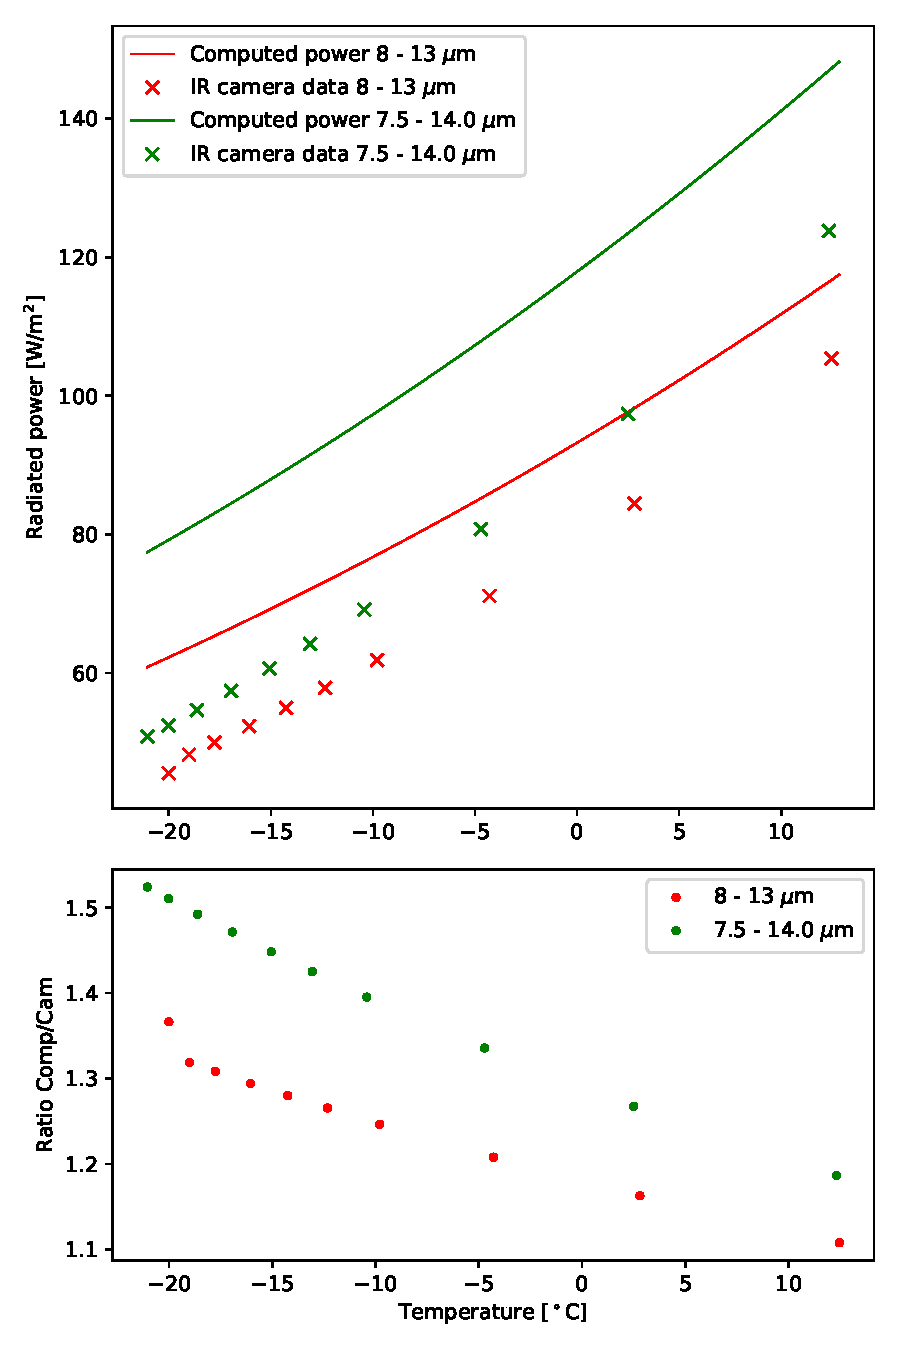
\includegraphics[width=0.65\textwidth]{img/T_to_P_Ranges.pdf}
	\caption{Testing with different wavelength ranges.}
	\label{fig:TempPowerRanges}
\end{figure}
\subsubsection{Different Emissivities}
Another try is varying the emissivity in the camera as shown in figure \ref{fig:TempPowerEps}. The lowest emissivity 0.90 appears to give the best model. Still, we do not want to settle with this result because shapewise, the curve for $\epsilon=1.00$ resembles the camera values most.
\begin{figure}[h!]
	\centering
	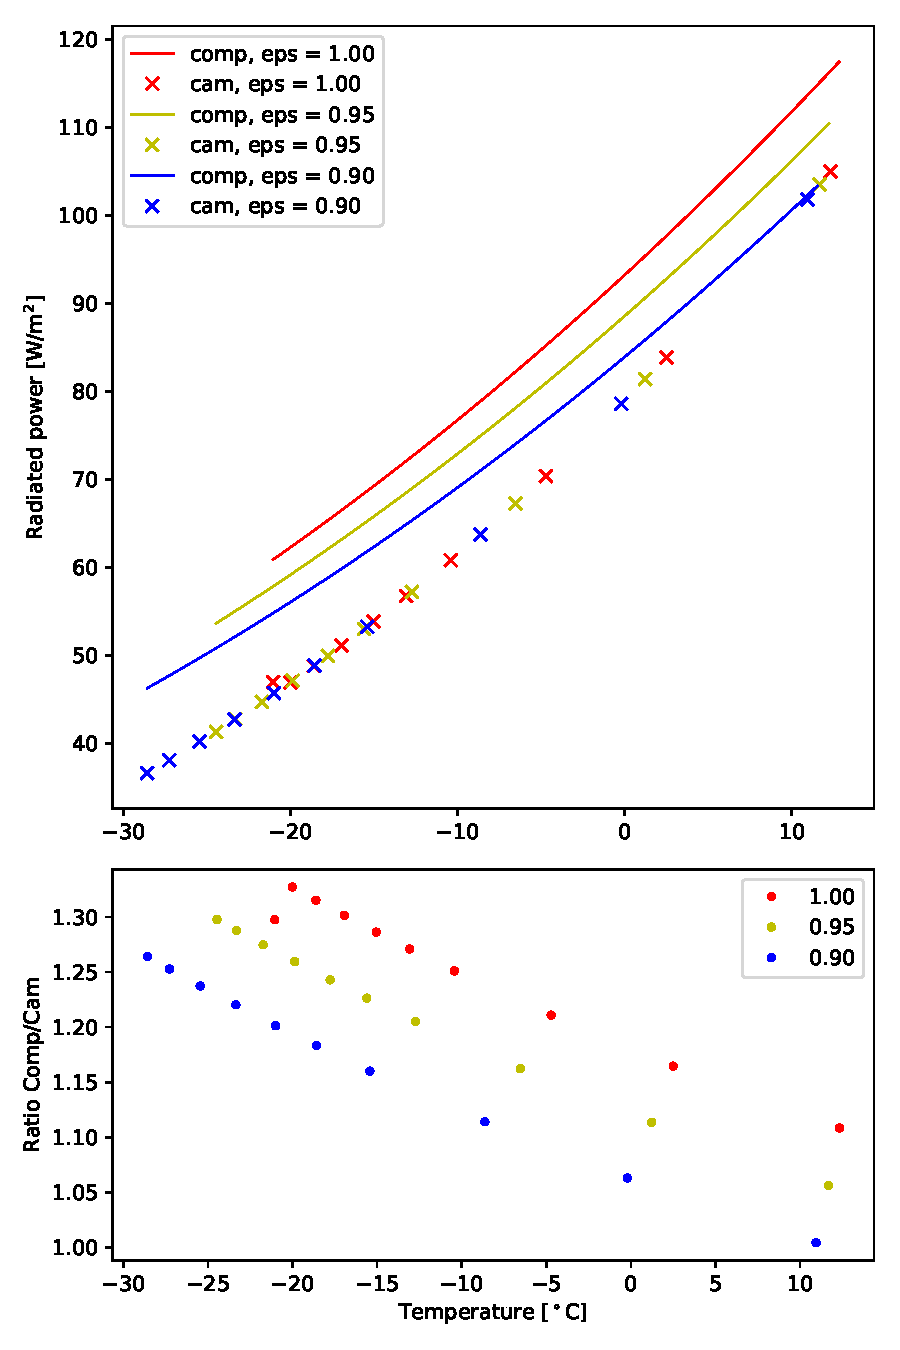
\includegraphics[width=0.65\textwidth]{img/T_to_P_Eps.pdf}
	\caption{Test with different emissivities.}
	\label{fig:TempPowerEps}
\end{figure}
\subsubsection{Fit with Global Scaling Factor}
\todo[noline]{Where does the idea with the global scaling factor come from? Wasn't it related to something about a Germanium detector?}
We also tried fitting the equation to the camera values using a global scaling parameter:
\begin{align}
	P(T) = \tau\left[\epsilon S(T) + (1-\epsilon)S(T_\text{amb})\right] \ .
\end{align}
In figure \ref{fig:TempPowerFit}, we see the fit obtained with the built in function \textsf{curve\_fit} of the \textsf{python} package \textsf{scipy.optimize}. Looking at the plot, one intuitively remarks that this does not seem to be the best fit. Interestingly, this computational deviation is not reflected by extremely high uncertainties:
\begin{align*}
	\tau_{1.00} &= 0.821\pm 0.018 \ , \\
	\tau_{0.95} &= 0.856\pm 0.021 \ , \\
	\tau_{0.90} &= 0.896\pm 0.024 \ . \\
\end{align*}
%The covariance matrix in table \ref{tab:pcov} reflects this assumption.
%\begin{table}[h!]
%	\centering
%	\begin{tabular}{l|ccccc}
%		& $\lambda_\text{min}$ [\si{\micro\metre}] & $\lambda_\text{max}$ [\si{\micro\metre}] & $T_\text{amb}$ [\si{\degreeCelsius}] & $\epsilon$ & $\tau$ \\
%		\hline
%		$\lambda_\text{min}$ & \SI{9.36e+03}{} & \SI{-1.17e+04}{} & \SI{2.46e-09}{} & \SI{1.33e+06}{} & \SI{-1.09e+06}{} \\
%		$\lambda_\text{max}$ & \SI{-1.17e+04}{} & \SI{1.47e+04}{} & \SI{-3.17e-09}{} & \SI{-1.77e+06}{} & \SI{1.40e+06}{} \\
%		$T_\text{amb}$ & \SI{2.46e-09}{} & \SI{-3.16e-09}{} & \SI{6.57e-21}{} & \SI{3.54e-06}{} & \SI{-2.91e-06}{} \\
%		$\epsilon$ & \SI{1.33e+06}{} & \SI{-1.71e+06}{} & \SI{3.54e-06}{} & \SI{1.90e+09}{} & \SI{-1.56e+09}{} \\
%		$\tau$ & \SI{-1.09e+06}{} & \SI{1.40e+06}{} & \SI{-2.91e-06}{} & \SI{-1.56e+09}{} & \SI{1.29e+09}{}
%	\end{tabular}
%	\caption{Covariance matrix for the fit with $\epsilon=1.00$.}
%	\label{tab:pcov}
%\end{table}
\begin{figure}[h!]
	\centering
	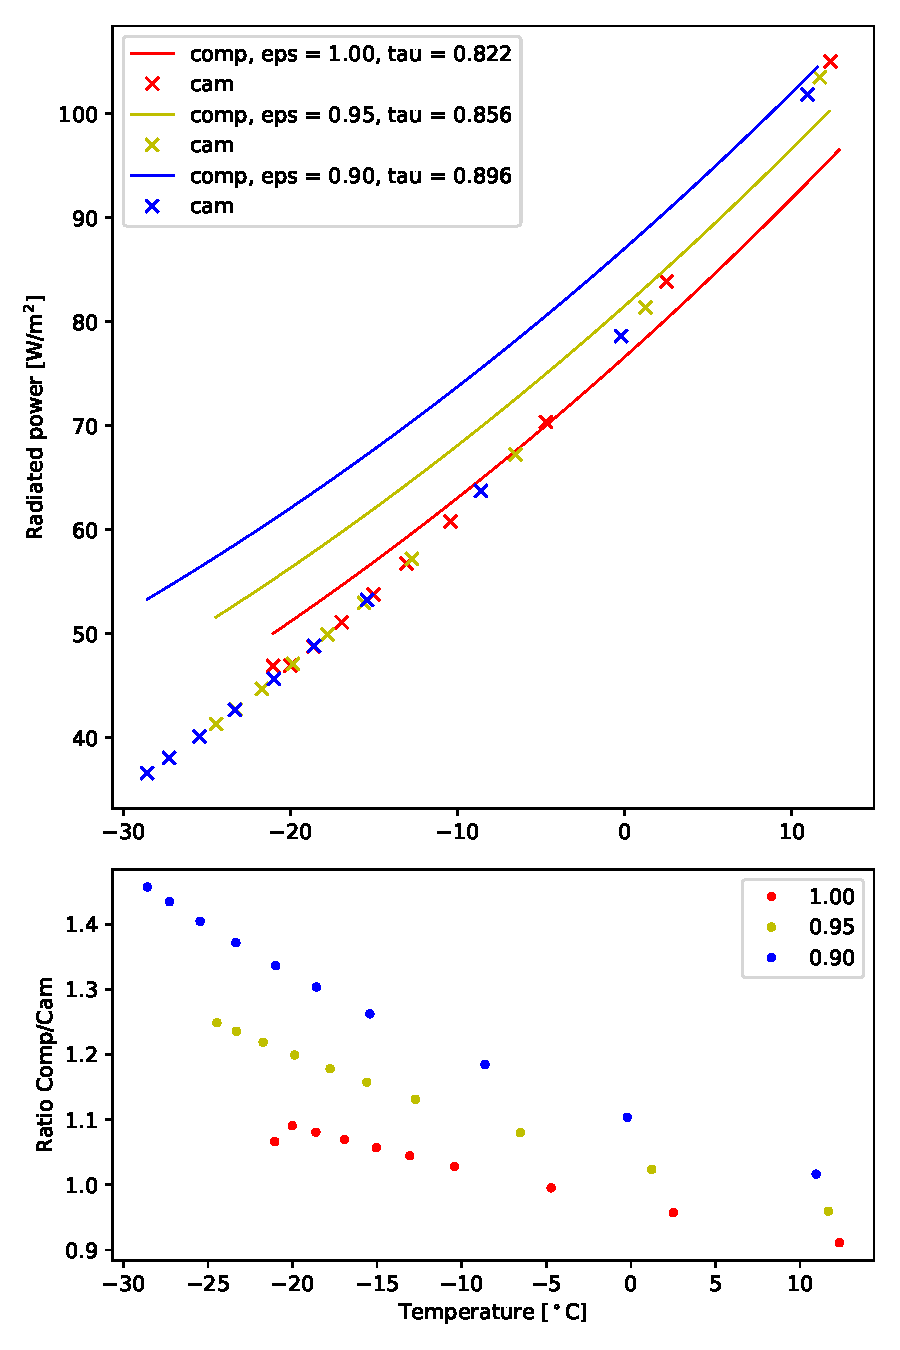
\includegraphics[width=0.6\textwidth]{img/T_to_P_Fit.pdf}
	\caption{Fitting the function to the camera values using a global scaling factor.}
	\label{fig:TempPowerFit}
\end{figure}